\chapter{境界条件から開弦のスペクトルへ}

\lectureoverview{我々の目的は開弦を量子化し、その状態が粒子と呼ばれるに値するかどうかを決定することである。道筋は初等的だが厳密を要する。まず\(0\leq\sigma\leq\pi\)上の関数の微積分とフーリエ解析を準備する。次に点粒子性を粒子挙動のスペクトル的判定基準で置き換え、横方向の力学が非相対論的になる無限運動量記述を復習し、軽い質量と剛いばねの連鎖から弦を構成する。連続弦は自由端点をもつ波動系である。そのノイマンモードは振動数\(1,2,3,\ldots\)の調和振動子に分離する。したがって量子化は離散的でギャップのあるスペクトルを生む。最後に弦の相互作用は我々を開弦の先へと押しやる。開弦はその両端点を結合して閉弦になりうる。}

\section{開弦区間上の微積分}

計算では離散和を積分に、最近接差分を微分に繰り返し変換することになる。それらが物理の邪魔をする前に、事実を整えておく方がよい。

\(x(\sigma)\)を

\begin{equation}
  0\leq \sigma\leq \pi .
\end{equation}

この記法は弦理論を先取りしている。\(\sigma\)は弦に沿った位置を表し、\(x\)はその横座標の一つになる。区間を\(N\)個に分割すると、

\begin{equation}
  \Delta\sigma=\frac{\pi}{N},
  \qquad
  \sigma_i=i\,\Delta\sigma,
  \qquad
  x_i=x(\sigma_i).
  \label{eq:l02-lattice}
\end{equation}

滑らかな極限関数に対して、

\begin{equation}
  \Delta x_i\equiv x_i-x_{i-1}
  =
  \frac{\partial x}{\partial\sigma}\,\Delta\sigma
  +O\!\left((\Delta\sigma)^2\right),
  \label{eq:l02-difference}
\end{equation}

であり、リーマン和は

\begin{equation}
  \sum_i x_i\,\Delta\sigma
  \longrightarrow
  \int_0^\pi x(\sigma)\,d\sigma .
  \label{eq:l02-riemann}
\end{equation}

\begin{figure}[H]
  \centering
  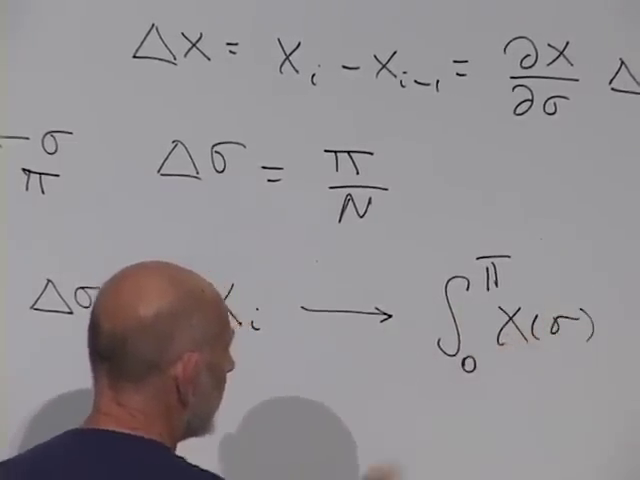
\includegraphics[width=0.78\textwidth]{lecture_02_figure_01.png}
  \caption{後の連続極限のために黒板に残された有限差分とリーマン和の規則。}
  \lectureframe{00:04:20}
  \label{fig:l02-calculus-board}
\end{figure}

これらは微積分でおなじみの定義である。ここでの重要性はスケーリングにある。\(\Delta x_i\)は\(\Delta\sigma\)の1乗をもたらすのに対し、和は積分になるとき1乗の逆数をもたらす。

\subsection{ディリクレ端点とノイマン端点}

有限区間上のフーリエ解析は端点での選択から始まる。二つの選択が繰り返し現れる。

\begin{align}
  \text{Dirichlet:}\qquad
  &x(0)=x(\pi)=0,
  \label{eq:l02-dirichlet}\\
  \text{Neumann:}\qquad
  &\left.\partial_\sigma x\right|_{\sigma=0}
   =
   \left.\partial_\sigma x\right|_{\sigma=\pi}
   =0.
  \label{eq:l02-neumann}
\end{align}

両端で保持されたバイオリン弦はディリクレの描像を与える。その変位は境界で消える。ノイマン関数はそこで消える必要はなく、各境界に傾きゼロで接する。二つの特徴的な形は黒板に一緒に見えている。

\begin{figure}[H]
  \centering
  \begin{minipage}[t]{0.48\textwidth}
    \centering
    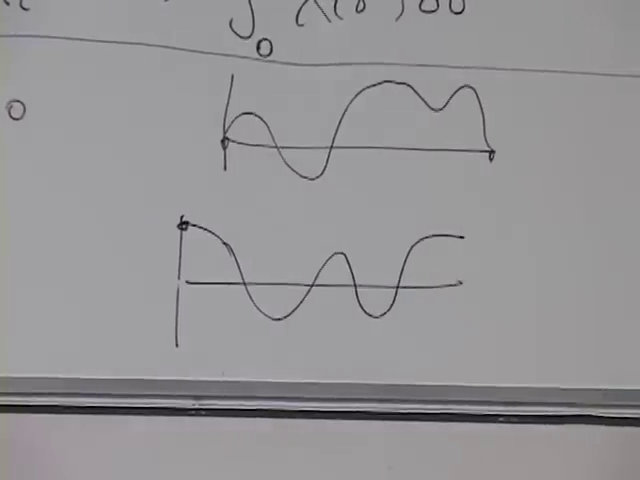
\includegraphics[width=\textwidth]{lecture_02_figure_02.png}
    \par\smallskip\footnotesize (a) 固定され平らな端点プロファイル。
  \end{minipage}\hfill
  \begin{minipage}[t]{0.48\textwidth}
    \centering
    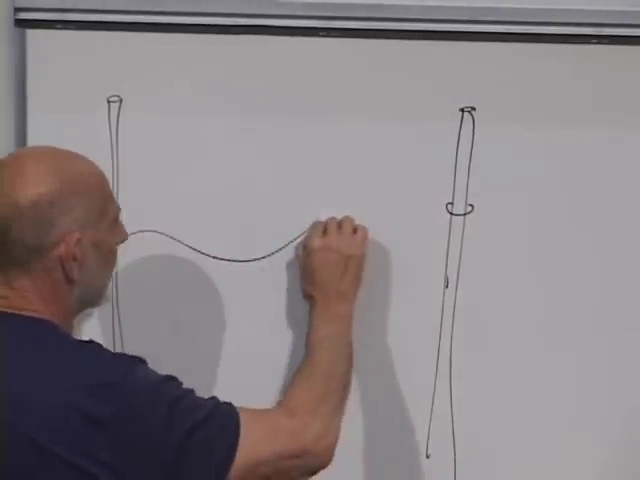
\includegraphics[width=\textwidth]{lecture_02_figure_03.png}
    \par\smallskip\footnotesize (b) 垂直なポール上を滑る軽いリング。
  \end{minipage}
  \caption{形として、また力学としての境界条件。滑りリングの構成は自由端点に曖昧さのない横方向の運動を与える。}
  \lectureframe{00:08:50 and 00:12:15}
  \label{fig:l02-boundaries-board}
\end{figure}

\begin{figure}[H]
  \centering
  \begin{adjustbox}{max width=\linewidth}
  \begin{tikzpicture}[>=Latex,thick,scale=0.92]
    \begin{scope}
      \draw[->] (0,0) -- (4.4,0) node[right] {\(\sigma\)};
      \draw[->] (0,-1.25) -- (0,1.35) node[above] {\(x\)};
      \draw[blue!70!black]
        (0,0) .. controls (0.8,1.1) and (1.4,1.0) .. (2.0,0)
        .. controls (2.7,-1.0) and (3.4,-0.8) .. (4.1,0);
      \fill (0,0) circle (0.06);
      \fill (4.1,0) circle (0.06);
      \node at (2.05,-1.65) {Dirichlet: \(x=0\)};
    \end{scope}
    \begin{scope}[xshift=5.8cm]
      \draw[->] (0,0) -- (4.4,0) node[right] {\(\sigma\)};
      \draw[->] (0,-1.25) -- (0,1.35) node[above] {\(x\)};
      \draw[orange!85!black]
        (0,0.65) .. controls (0.8,0.65) and (1.1,-0.9) .. (2.0,-0.9)
        .. controls (2.9,-0.9) and (3.2,0.55) .. (4.1,0.55);
      \draw[orange!85!black] (0,0.65) -- (0.45,0.65);
      \draw[orange!85!black] (3.65,0.55) -- (4.1,0.55);
      \node at (2.05,-1.65) {Neumann: \(\partial_\sigma x=0\)};
    \end{scope}
  \end{tikzpicture}
  \end{adjustbox}
  \caption{値はディリクレデータに対して固定され、傾きはノイマンデータに対して固定される。}
  \label{fig:l02-boundaries-redraw}
\end{figure}

\begin{classroomqa}
\audiencequestion{開管または閉管は、これらの境界条件の一方の明快な例を与えるか。\lecturetimestamp{00:09:19}}
\lecturerresponse{与えうるが、まずどの音響変数を展開するかを言わねばならない。圧力摂動と縦方向変位は開端で相補的な理想化条件に従う。その脇の問いを黒板で決着させるよりも、滑りリング模型を使う方がよい。ほとんど質量のないリングはポール上を垂直に動けるので、弦の端点は自由であり、ノイマンの描像は直接的である。}
\end{classroomqa}

\begin{classroomqa}
\audiencequestion{グラフは垂直に立ち上がり、鋭い跳びを含むことができるか。\lecturetimestamp{00:09:53}}
\lecturerresponse{フーリエ解析は区分的連続関数における孤立した跳びを許す。物理的な弦はより制限的である。跳びは隣接する点を切り離し、空間微分\(\partial_\sigma x\)を以下で導かれる連続エネルギーにおいて特異にする。したがって我々は連続かつ微分可能なプロファイルに注意を限定する。}
\end{classroomqa}

\begin{classroomqa}
\audiencequestion{なぜ管の開端、あるいは任意の自由端がそもそも境界条件を満たすべきなのか。\lecturetimestamp{00:11:14}}
\lecturerresponse{音響の例は選ばれた場に依存し、議論では未解決のまま残された。力学の例はそうではない。非常に軽いリングは滑ることは自由だが、それでも最後の弦の断片に取り付けられている。我々はその条件を仮定するのではなくニュートンの法則から導く。有限の端点加速度が傾きをゼロに強制する。}
\end{classroomqa}

\subsection{フーリエ基底}

端点のクラスが固定されれば、対応するフーリエ基底も固定される。\(0\leq\sigma\leq\pi\)上では、

\begin{align}
  x_D(\sigma)
  &=
  \sum_{n=1}^{\infty}x_n\sin(n\sigma),
  \label{eq:l02-dirichlet-series}\\
  x_N(\sigma)
  &=
  \sum_{n=0}^{\infty}x_n\cos(n\sigma).
  \label{eq:l02-neumann-series}
\end{align}

\eqref{eq:l02-dirichlet-series}のすべての正弦は両端点で消える。\eqref{eq:l02-neumann-series}のすべての余弦は端点微分がゼロである。下限が異なるのには理由がある。\(\sin(0\sigma)=0\)は何も寄与せず、\(\cos(0\sigma)=1\)は定数モード、すなわちゼロモードである。それはノイマン関数の平均値を記録する。

\begin{figure}[H]
  \centering
  \begin{minipage}[t]{0.48\textwidth}
    \centering
    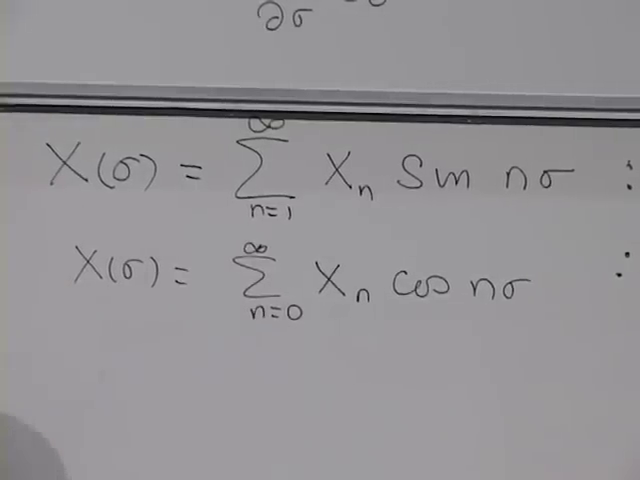
\includegraphics[width=\textwidth]{lecture_02_figure_04.png}
    \par\smallskip\footnotesize (a) 正弦展開と余弦展開。
  \end{minipage}\hfill
  \begin{minipage}[t]{0.48\textwidth}
    \centering
    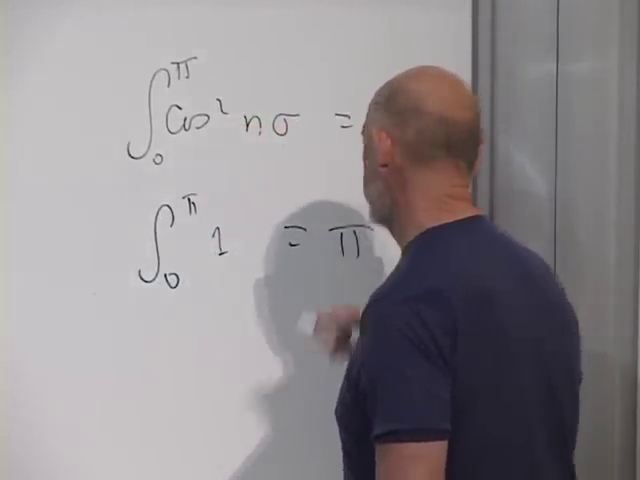
\includegraphics[width=\textwidth]{lecture_02_figure_05.png}
    \par\smallskip\footnotesize (b) 直交性と例外的な
    定数モード。
  \end{minipage}
  \caption{後に弦を対角化するために用いられるフーリエの事実。}
  \lectureframe{00:16:15 and 00:20:30}
  \label{fig:l02-fourier-board}
\end{figure}

微分はこの二つのクラスを入れ替える：

\begin{equation}
  \begin{aligned}
    \partial_\sigma\sin(n\sigma)&=n\cos(n\sigma),\\
    \partial_\sigma\cos(n\sigma)&=-n\sin(n\sigma).
  \end{aligned}
  \label{eq:l02-basis-derivatives}
\end{equation}

したがって、ディリクレ級数の導関数はノイマン的振る舞いを示し、ノイマン級数の導関数はディリクレ的振る舞いを示す。すると直交性により、異なるモード間の交差項が消える：

\begin{align}
  \int_0^\pi\cos(n\sigma)\cos(m\sigma)\,d\sigma
  &=
  \frac{\pi}{2}\delta_{nm},
  && n,m\geq1,
  \label{eq:l02-cos-orthogonality}\\
  \int_0^\pi\sin(n\sigma)\sin(m\sigma)\,d\sigma
  &=
  \frac{\pi}{2}\delta_{nm},
  && n,m\geq1,
  \label{eq:l02-sin-orthogonality}\\
  \int_0^\pi 1\,d\sigma&=\pi .
  \label{eq:l02-zero-norm}
\end{align}

最後の行は例外的な\(n=m=0\)余弦ノルムである。定数は非零の調和振動子のようには規格化されず、この因子2が弦の重心モードを内部モードから区別することになる。

\subsection{覚えておくべき振動子の公式}

座標を再スケールしてその力学的質量を1にすると、フックの法則に従う振動子は次を持つ

\begin{align}
  E_{\mathrm{osc}}
  &=
  \frac12\dot q^{\,2}
  +\frac12\omega^2q^2,
  \label{eq:l02-oscillator-energy}\\
  L_{\mathrm{osc}}
  &=
  \frac12\dot q^{\,2}
  -\frac12\omega^2q^2.
  \label{eq:l02-oscillator-lagrangian}
\end{align}

\begin{figure}[H]
  \centering
  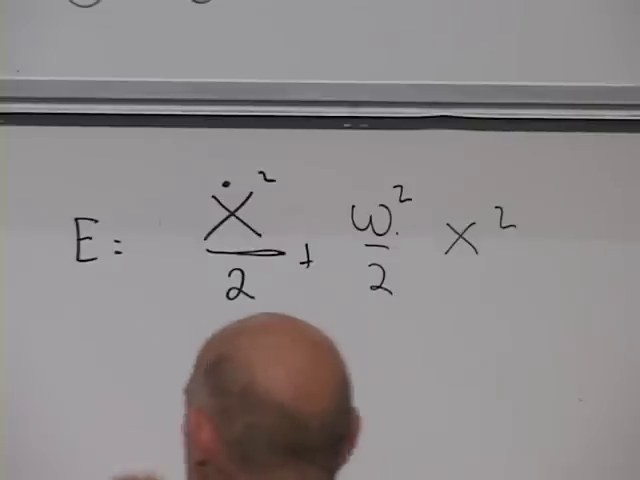
\includegraphics[width=0.68\textwidth]{lecture_02_figure_06.png}
  \caption{振動子のエネルギー。\(q^2\)の係数が直ちに\(\omega^2\)を同定するように書かれている。}
  \lectureframe{00:24:00}
  \label{fig:l02-oscillator-board}
\end{figure}

古典的には\(\omega=\sqrt{\kappa/m}\)であり、座標の再スケーリングにより\(m=1\)が設定されている。量子力学的には、

\begin{equation}
  E_Q=\hbar\omega\left(Q+\frac12\right),
  \qquad Q=0,1,2,\ldots .
  \label{eq:l02-oscillator-spectrum}
\end{equation}

準位間隔については、共通の基底状態の項を差し引いて、各量子が\(\hbar\omega\)のコストを要すると言ってよい。弦の計算では最初にまさにそうし、全零点エネルギーは後回しにする。

\begin{classroomqa}
\audiencequestion{振動子の振動数はエネルギー公式からどのように読み取られるのか。\lecturetimestamp{00:23:21}}
\lecturerresponse{再スケーリング前は\(\omega=\sqrt{\kappa/m}\)である。単位質量ではポテンシャル項は\(\frac12\omega^2q^2\)なので、その二次の係数が振動数の二乗である。}
\end{classroomqa}

\section{複合系を粒子たらしめるものは何か。}

弦は拡がっており、多数の結合した部分によってモデル化される。それにもかかわらず、その量子状態の一つが粒子でありうるのはどのような意味においてか。点状であることは決定的な基準にはなりえない。陽子と中性子は複合系である。電子と光子は、固有の内部構造が解明されていないにもかかわらず、量子場の衣をまとっている。何にも囲まれていない古典的な幾何学的点は、量子励起の正しい像ではない。

質量と重心の位置も十分ではない。密閉された気体の箱はその両方を持つ。コーヒーカップもその両方を持つ。我々は通常、どちらも粒子とは呼ばない。不可分性もまた成り立たない。陽子は可分だからである。そしてスピンは微視的粒子と巨視的物体を区別しない。

有用な基準はスペクトルの孤立性である。静止エネルギーを縦軸に取り、別の内部状態に到達するのにどれだけのエネルギーが必要かを問う。電子には、そのすぐ上に実験的に到達可能な電子励起の塔はない。陽子には共鳴状態が確かにあるが、最初のものは数百MeVを要し、陽子質量のかなりの割合である。それらの状態は個別に同定できるほど十分に離れている。

コーヒーカップは逆である。長波長の音響モードに任意に小さなエネルギーを加えたり、分子をわずかに揺らしたり、フォノンを生成したりできる。膨大な数の状態が微小な間隔に詰め込まれている。実験室のスケールではそれらは連続体をなす。これが粒子と\emph{マッシュ}の実用的な区別である。

\begin{figure}[H]
  \centering
  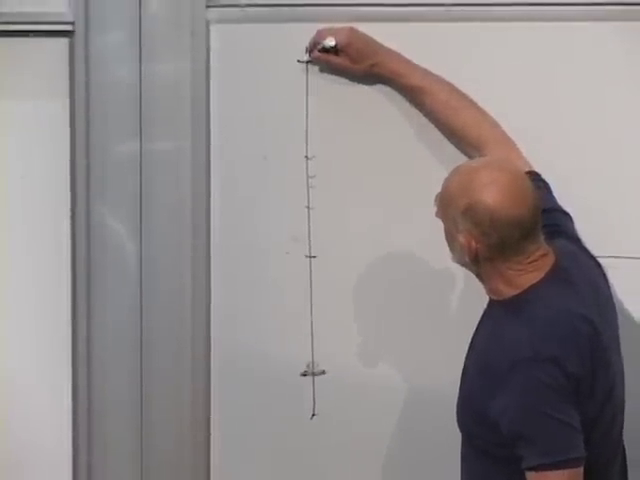
\includegraphics[width=0.58\textwidth]{lecture_02_figure_07.png}
  \caption{孤立した粒子準位と通常の物質の密な励起を比較する際の、黒板上の縦軸のエネルギー軸。}
  \lectureframe{00:31:10}
  \label{fig:l02-spectrum-board}
\end{figure}

\begin{figure}[H]
  \centering
  \begin{adjustbox}{max width=\linewidth}
  \begin{tikzpicture}[>=Latex,thick]
    \begin{scope}
      \draw[->] (0,0) -- (0,4.8) node[above] {energy};
      \draw[blue!70!black,line width=1.2pt] (-1.0,0.65) -- (1.0,0.65);
      \draw[blue!70!black,line width=1.2pt] (-1.0,3.65) -- (1.0,3.65);
      \node[right] at (1.05,0.65) {ground state};
      \node[right] at (1.05,3.65) {first internal excitation};
      \draw[<->] (0.65,0.75) -- (0.65,3.55)
        node[midway,right] {large gap};
      \node at (0,-0.55) {particle-like};
    \end{scope}
    \begin{scope}[xshift=7.0cm]
      \draw[->] (0,0) -- (0,4.8) node[above] {energy};
      \foreach \y in {0.55,0.69,0.82,0.94,1.05,1.15,1.24,1.32,1.39,1.45,
        1.51,1.57,1.63,1.70,1.78,1.87,1.97,2.09,2.22,2.36,2.51,2.67,2.84,
        3.02,3.21,3.41,3.62,3.84,4.07}
        \draw[orange!85!black] (-0.95,\y) -- (0.95,\y);
      \node[right] at (1.05,2.25) {dense phonon and internal states};
      \node at (0,-0.55) {macroscopic matter};
    \end{scope}
  \end{tikzpicture}
  \end{adjustbox}
  \caption{講義で用いられる操作的な粒子基準は、文字通りの点状性ではなくスペクトルの孤立性である。}
  \label{fig:l02-particle-redraw}
\end{figure}

この基準は哲学的問いを計算に変える。弦を量子化し、その内部エネルギー準位を求め、それらの間隔を調べる。もし最初の励起弦状態がプランクスケール付近にあり、観測される基底状態が軽いならば、そのギャップは現在の加速器エネルギーを二十桁以上も超えている。そのとき弦は、到達可能な領域の全体にわたって素粒子のように振る舞う。

\begin{classroomqa}
\audiencequestion{粒子の振る舞いは単に観測スケールの問題にすぎないのか。十分に拡大すれば、準位はもはや分離しなくなるのか。\lecturetimestamp{00:33:33}}
\lecturerresponse{拡大すれば物体が多くの構成要素を持つことが明らかになるかもしれないが、スペクトルが消えるわけではない。関連する比較は、実験のエネルギー分解能と最初の内部励起までのギャップとの間にある。そのギャップが膨大であれば、複合的な物体も粒子のように振る舞い続けうる。}
\end{classroomqa}

\begin{classroomqa}
\audiencequestion{なぜ普通のバイオリン弦は粒子ではないのか。\lecturetimestamp{00:34:37}}
\lecturerresponse{1つの振動量子が運ぶエネルギーは、巨視的な弦の静止エネルギーに比べて測定不能なほど小さい。したがって多くの量子状態がごくわずかな相対的間隔に収まる。これはスペクトル比較において孤立した側ではなく、密な側に属する。}
\end{classroomqa}

\begin{classroomqa}
\audiencequestion{量子場が仮想的な揺らぎで光子や電子を取り囲んでいるならば、それらは点粒子なのか。\lecturetimestamp{00:35:40}}
\lecturerresponse{古典的な語\emph{点}はあまりに多くの役割を負わされている。物理的な電子と光子はドレスされた場の励起であるが、実験はどちらについても内在的な構成要素構造や有限の形状因子を発見していない。現在の議論にとって重要なのは、どちらもほとんど縮退した内部状態の密な塔を持たないことである。\editorialnote{この講義は電子の異常磁気モーメントを測定可能な量子的な揺らぎと結びつけている。現代の用語では、異常モーメントは輻射的ドレッシング効果であり、分解された有限の電子半径の証拠ではない。点状とは慣例的に、試験されたスケールまで内在的な下部構造や形状因子が検出されていないことを意味する。}}
\end{classroomqa}

\begin{classroomqa}
\audiencequestion{光子の大きさはその振動数に依存するのか。\lecturetimestamp{00:36:49}}
\lecturerresponse{その波長は確かに依存する。それは内在的な構成要素の大きさとは別である。振動数を変えると波束と波長が変わるのであり、光子の分解された内部半径が変わるのではない。}
\end{classroomqa}

\section{大きな運動量における厳密な横方向の力学}

ここで相対論的な困難に戻る。高速で回転する棒は、その重心を静止させるだけでは非相対論的に扱えない。その両端は依然として互いに対して相対論的に運動している。非相対論的近似が破れるのは、内部の相対運動のためである。

しかしながら、別の極限が存在する。\(z\)軸を選び、系全体を非常に大きな正の縦方向運動量\(P_z\)へブーストする。その横方向運動量を

\begin{equation}
  p_\perp^2=p_x^2+p_y^2
\end{equation}

有限に保つ。すると横方向射影は、\(P_z\to\infty\)極限において厳密に非相対論的なハミルトニアンの形を許容する。たとえブーストされていない内部運動が相対論的であったとしてもである。

\begin{classroomqa}
\audiencequestion{無限大の運動量とは、質量を持つ系が実際に光速に達することを意味するのか。\lecturetimestamp{00:40:43}}
\lecturerresponse{いかなる有限のブーストもそれには達しない。\(P_z\)がいくらでも大きくなるときに、よく定義された極限を持つ量を構成する。この語句は極限操作を名指すのであり、\(v=c\)を持つ有限の物理的状態を名指すのではない。}
\end{classroomqa}

\begin{classroomqa}
\audiencequestion{どの軸を選ぶべきか、また物体がその軸のまわりを、あるいはその軸を横切って回転する場合はどうか。\lecturetimestamp{00:41:14}}
\lecturerresponse{任意の軸を選んでよく、系全体をそれに沿ってブーストする。明示的な力学として残るのは、垂直な平面への射影である。回転する棒は短縮されて見えたり、その平面を掃いたりするかもしれないが、その横方向射影は非相対論的な形を持つ。}
\end{classroomqa}

弦には、この表現を異常に強力にする追加の性質がある。光円錐ゲージでは、その縦方向の内部座標は独立な振動子ではない。拘束条件がそれらを横方向の運動から決定する。したがって横方向の弦を知れば、物理的自由度を再構成するのに十分である。

\begin{classroomqa}
\audiencequestion{独立な縦方向座標が存在しないということは、弦が単に薄いサンドイッチの中に閉じ込められているということを意味するのか。\lecturetimestamp{00:42:26}}
\lecturerresponse{ローレンツ収縮は確かにブーストされた系においてその縦方向の広がりを小さくするが、この主張はそれよりも強い。残存する縦方向の運動は横方向の運動によって拘束され、独立に指定することはできない。}
\end{classroomqa}

\begin{classroomqa}
\audiencequestion{この横方向のデータへの還元はホログラフィック原理と関係があるのか。\lecturetimestamp{00:43:12}}
\lecturerresponse{それはホログラフィックな考え方に至った思考の流れと密接に関係しているが、その関係を追及することは現在の計算から離れてしまう。ここでは横方向の弦を扱うことを正当化する役割しか果たさない。}
\end{classroomqa}

\subsection{ブーストの差し引きと時間の再スケーリング}

\(M\)を、構成要素の質量、運動エネルギー、束縛エネルギーを含む系全体の不変質量とする。単位\(c=1\)では、

\begin{equation}
  E=\sqrt{P_z^2+p_\perp^2+M^2}.
  \label{eq:l02-relativistic-energy}
\end{equation}

\(P_z\)が\(p_\perp\)および\(M\)よりもずっと大きいとき、

\begin{equation}
  E
  =
  P_z+\frac{p_\perp^2+M^2}{2P_z}
  +O(P_z^{-3}).
  \label{eq:l02-large-pz}
\end{equation}

\begin{figure}[H]
  \centering
  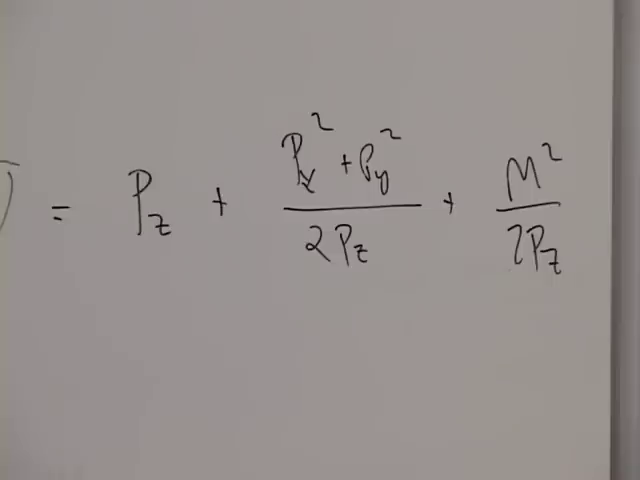
\includegraphics[width=0.76\textwidth]{lecture_02_figure_08.png}
  \caption{横方向運動量と不変質量を保持した、完成された大きな\(P_z\)展開。}
  \lectureframe{00:47:30}
  \label{fig:l02-large-pz-board}
\end{figure}

主要項は大きいが、内部状態に関する情報を何も運んでいない。\(P_z\)を保存する過程、たとえば全縦運動量を変えずに内部準位間を遷移するブーストされた原子のような過程では、この項はすべてのエネルギー差から相殺される。したがって我々は次を調べる。

\begin{equation}
  E-P_z=\frac{p_\perp^2+M^2}{2P_z}+O(P_z^{-3}).
  \label{eq:l02-residual-energy}
\end{equation}

分母には物理的な意味がある。ハミルトニアンが時間発展を生成するので、小さな残留エネルギーは、内部発展が実験室時間では遅く見えることを述べている。これが時間の遅れである。内部運動を保つために、再スケールされた発展パラメータ\(\tau\)を導入する。あるいは同等に、残留ハミルトニアンに\(P_z\)を掛ける。

\begin{equation}
  H_\perp
  \equiv
  \lim_{P_z\to\infty}P_z(E-P_z)
  =
  \frac12p_\perp^2+\frac12M^2.
  \label{eq:l02-transverse-hamiltonian}
\end{equation}

\begin{figure}[H]
  \centering
  \begin{minipage}[t]{0.48\textwidth}
    \centering
    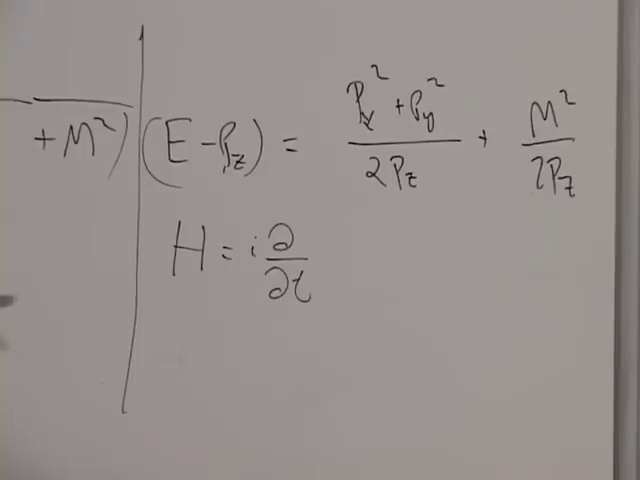
\includegraphics[width=\textwidth]{lecture_02_figure_09.png}
    \par\smallskip\footnotesize (a) \(H=i\partial_t\)と、遅くなった内部発展。
  \end{minipage}\hfill
  \begin{minipage}[t]{0.48\textwidth}
    \centering
    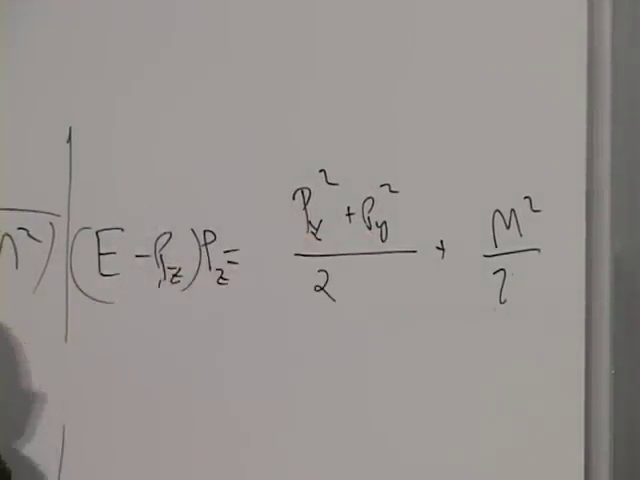
\includegraphics[width=\textwidth]{lecture_02_figure_10.png}
    \par\smallskip\footnotesize (b) 時間再スケーリング後の有限な横方向ハミルトニアン。
  \end{minipage}
  \caption{時間の遅れた残留エネルギーから有限な二次元ハミルトニアンへ。}
  \lectureframe{00:49:20 and 00:52:40}
  \label{fig:l02-lightfront-board}
\end{figure}

これはまさに、二次元を運動する単位質量粒子の形である。運動エネルギー\(p_\perp^2/2\)に内部エネルギー\(M^2/2\)を加えたものである。珍しい特徴はその二乗である。この記述では、静止エネルギーすなわち束縛エネルギーの役割を果たす量は、不変質量の二乗に比例する。\editorialnote{従来の光円錐変数\(P^\pm=(E\pm P_z)/\sqrt2\)を用いると、厳密な質量殻関係は\(2P^+P^-=p_\perp^2+M^2\)である。式\eqref{eq:l02-transverse-hamiltonian}は、同じ不変関係のこの講義における大きな\(P_z\)の規格化である。}

\begin{classroomqa}
\audiencequestion{複合系の個々の部分の縦運動量はどうなったのか。\lecturetimestamp{00:51:30}}
\lecturerresponse{一般的な複合物体では、その構成要素が担う全\(P_z\)の割合を保持しなければならない。上の式は全重心運動量を用いている。弦理論が特別なのは、その拘束条件が横方向の自由度から相対的な縦運動を決定するため、独立な縦方向振動子を加える必要がないからである。}
\end{classroomqa}

\section{離散的な開弦}

ブーストされた弦は今や明示的に横平面内だけを運動する。その二つの座標を\(X\)および\(Y\)と名付け、まずそれを\(N-1\)本のばねで結ばれた\(N\)個の質点で近似する。\(\mu\)を各点の対応する質量、\(k\)を最近接ばね定数とすると、エネルギーは次である。

\begin{equation}
  E_N
  =
  \sum_i
  \left[
    \frac{\mu}{2}
    \left(\dot X_i^2+\dot Y_i^2\right)
    +
    \frac{k}{2}
    \left((\Delta X_i)^2+(\Delta Y_i)^2\right)
  \right].
  \label{eq:l02-discrete-energy}
\end{equation}

横平面には二つの方向があるので、すべての\(X\)項には同一の\(Y\)項が対応する。添字\(i\)は鎖に沿った点を表し、空間座標ではない。

\begin{figure}[H]
  \centering
  \begin{minipage}[t]{0.48\textwidth}
    \centering
    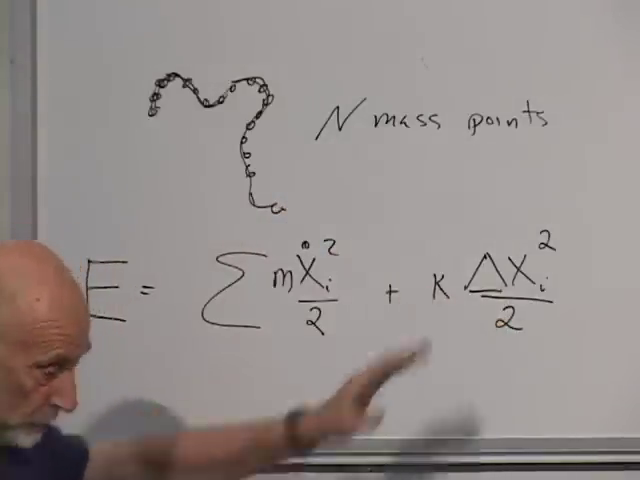
\includegraphics[width=\textwidth]{lecture_02_figure_11.png}
    \par\smallskip\footnotesize (a) ビーズ鎖とその離散エネルギー。
  \end{minipage}\hfill
  \begin{minipage}[t]{0.48\textwidth}
    \centering
    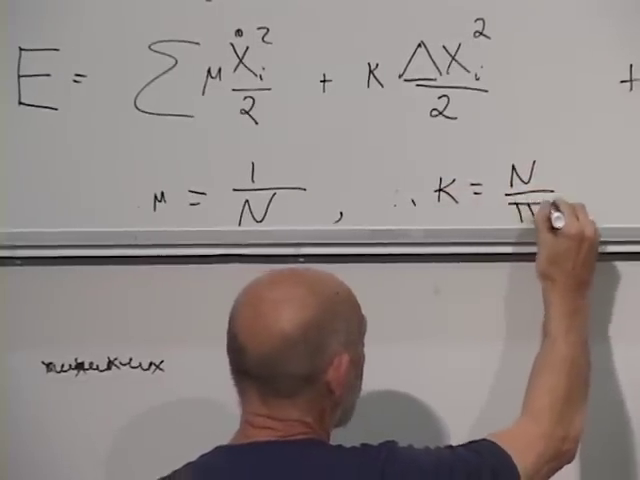
\includegraphics[width=\textwidth]{lecture_02_figure_12.png}
    \par\smallskip\footnotesize (b) \(\mu\)と\(k\)の大きな\(N\)でのスケーリング。
  \end{minipage}
  \caption{連続極限を取る前の正則化された開弦。}
  \lectureframe{00:57:42 and 01:02:40}
  \label{fig:l02-chain-board}
\end{figure}

\begin{figure}[H]
  \centering
  \begin{adjustbox}{max width=\linewidth}
  \begin{tikzpicture}[>=Latex,thick]
    \foreach \i in {0,...,8} {
      \coordinate (p\i) at ({1.05*\i},{0.30*sin(55*\i)});
      \filldraw[white] (p\i) circle (0.10);
      \draw (p\i) circle (0.10);
    }
    \foreach \i in {0,...,7} {
      \pgfmathtruncatemacro{\j}{\i+1}
      \draw[decorate,decoration={zigzag,segment length=4pt,amplitude=2pt}]
        (p\i) -- (p\j);
    }
    \node[above=0.35cm of p0] {\(i=0\)};
    \node[above=0.35cm of p8] {\(i=N-1\)};
    \draw[<->] (0,-1.15) -- (8.4,-1.15)
      node[midway,below] {\(0\leq\sigma\leq\pi\)};
    \node at (4.2,1.25)
      {\(\mu=1/N,\quad k=N/\pi^2,\quad\Delta\sigma=\pi/N\)};
  \end{tikzpicture}
  \end{adjustbox}
  \caption{明快な正則化の描像。鎖を細かくするにつれて、点は軽くなり、微視的なばねは硬くなる。}
  \label{fig:l02-chain-redraw}
\end{figure}

パラメータ\(\sigma\)は鎖に沿った位置を表す。\(0\leq\sigma\leq\pi\)を選ぶのは慣習であり、物理的な長さの測定ではない。これは弦が二つの端点をもつことを思い起こさせる。後に閉弦は\(0\leq\sigma<2\pi\)上で周期的にラベル付けされる。

連続極限は集団的力学を有限に保たなければならない。ビーズの質量を固定すると全対応質量が発散するので、次を選ぶ。

\begin{equation}
  \mu=\frac{1}{N}.
  \label{eq:l02-mu-scaling}
\end{equation}

すると\(N\mu=1\)となる。これは相対論的な静止質量\(M\)ではなく、横方向対応模型における慣性係数である。

直列のばねはその数が増えるにつれて柔らかくなる。鎖全体の剛性を有限に保つには、各微視的ばねが硬くならなければならない。

\begin{equation}
  k=\frac{N}{\pi^2}
  =\frac{1}{\pi\,\Delta\sigma}.
  \label{eq:l02-k-scaling}
\end{equation}

本質的なのは\(k\propto N\)だけである。\(\pi^2\)の因子は、連続体の式から余分な\(\pi\)の因子を取り除くために選ばれた規格化である。

\begin{classroomqa}
\audiencequestion{\(\mu\)は各弦点の物理的な静止質量か。\lecturetimestamp{01:10:34}}
\lecturerresponse{いいえ。それは横方向の鎖に現れる非相対論的な対応質量である。それを\(M\)と呼ぶと、相対論的な弦状態全体の不変静止質量と混同することになる。現在の唯一の役割は、正しい連続体の慣性を生み出すことである。}
\end{classroomqa}

\section{連続体の波動系}

最初に用意した規則を適用する。\(1/N=\Delta\sigma/\pi\)なので、

\begin{align}
  \sum_i\frac{\mu}{2}\dot X_i^2
  &=
  \frac{1}{2\pi}
  \sum_i\dot X_i^2\,\Delta\sigma
  \longrightarrow
  \frac{1}{2\pi}
  \int_0^\pi
  \left(\partial_\tau X\right)^2d\sigma ,
  \label{eq:l02-kinetic-limit}\\
  \sum_i\frac{k}{2}(\Delta X_i)^2
  &\longrightarrow
  \frac{1}{2\pi}
  \int_0^\pi
  \left(\partial_\sigma X\right)^2d\sigma .
  \label{eq:l02-potential-limit}
\end{align}

第二行には、\(\Delta X_i=\partial_\sigma X\,\Delta\sigma\)を\(k=1/(\pi\Delta\sigma)\)とともに用いる。同じ計算は\(Y\)にも当てはまる。

\begin{figure}[H]
  \centering
  \begin{minipage}[t]{0.48\textwidth}
    \centering
    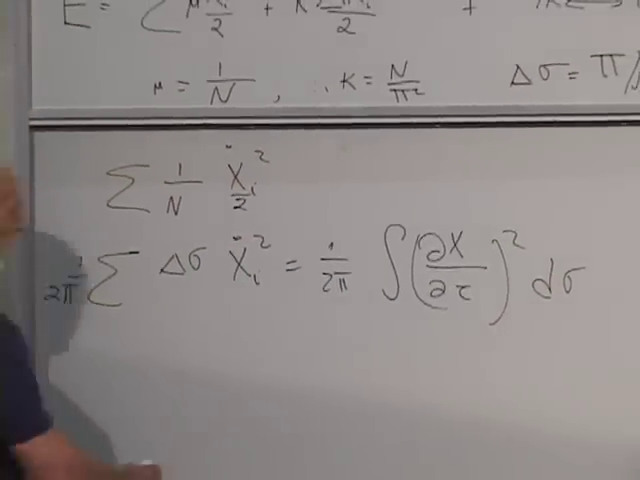
\includegraphics[width=\textwidth]{lecture_02_figure_13.png}
    \par\smallskip\footnotesize (a) 和から積分への置き換えと
    差から微分への置き換え。
  \end{minipage}\hfill
  \begin{minipage}[t]{0.48\textwidth}
    \centering
    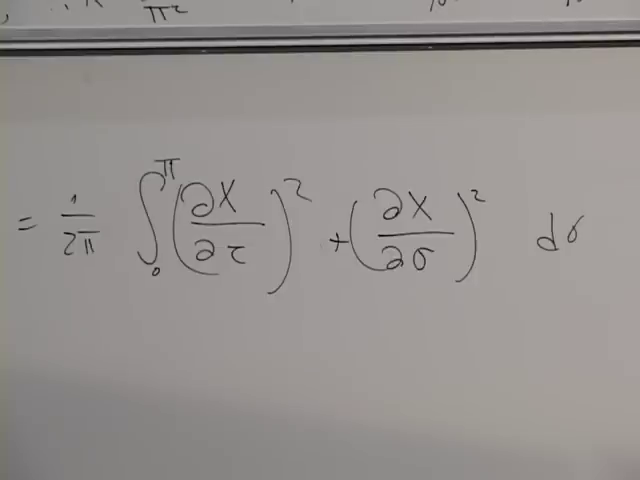
\includegraphics[width=\textwidth]{lecture_02_figure_14.png}
    \par\smallskip\footnotesize (b) 完成した連続極限のエネルギー。
  \end{minipage}
  \caption{離散的な鎖が\(\sigma\)区間上の場になる。}
  \lectureframe{01:05:40 and 01:07:00}
  \label{fig:l02-continuum-board}
\end{figure}

得られるエネルギーとラグランジアンは

\begin{align}
  E
  &=
  \frac{1}{2\pi}
  \int_0^\pi d\sigma\,
  \left[
    (\partial_\tau X)^2+(\partial_\tau Y)^2\right.\notag\\[-0.25em]
  &\hspace{6.5em}\left.
    +(\partial_\sigma X)^2+(\partial_\sigma Y)^2
  \right],
  \label{eq:l02-continuum-energy}\\
  L
  &=
  \frac{1}{2\pi}
  \int_0^\pi d\sigma\,
  \left[
    (\partial_\tau X)^2+(\partial_\tau Y)^2\right.\notag\\[-0.25em]
  &\hspace{6.5em}\left.
    -(\partial_\sigma X)^2-(\partial_\sigma Y)^2
  \right].
  \label{eq:l02-continuum-lagrangian}
\end{align}

\begin{figure}[H]
  \centering
  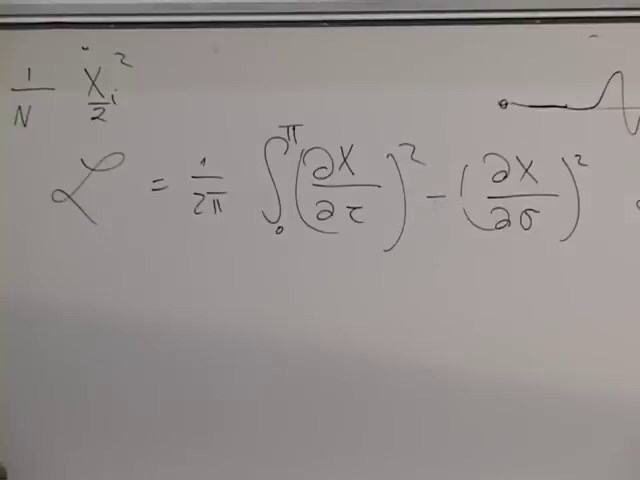
\includegraphics[width=0.78\textwidth]{lecture_02_figure_15.png}
  \caption{運動項と伸長項が逆符号を持つ連続極限のラグランジアン。}
  \lectureframe{01:08:48}
  \label{fig:l02-lagrangian-board}
\end{figure}

\(\sigma\)を通常の空間座標、\(X\)を場\(\phi\)と名付け直せば、これらは一次元波動場のエネルギーとラグランジアンである。\eqref{eq:l02-continuum-lagrangian}を変分すると

\begin{equation}
  \left(\partial_\tau^2-\partial_\sigma^2\right)X=0,
  \qquad
  \left(\partial_\tau^2-\partial_\sigma^2\right)Y=0.
  \label{eq:l02-wave-equation}
\end{equation}

当面の議論では、これらの方程式を直接解く必要はない。有用な描像は、波が弦に沿って左右に伝わり、端点で反射するというだけのことである。ディリクレ反射は変位の符号を反転させ、ノイマン反射はそれを保つ。

\begin{classroomqa}
\audiencequestion{時間変数\(\tau\)とは正確には何か。\lecturetimestamp{01:08:54}}
\lecturerresponse{それは、大\(P_z\)極限の記述で内部運動を追うために用いられる、再スケールされた時間である。系とともにブーストされた時計は実験室時間に対して遅く進むが、\(\tau\)はその遅れを取り除くので、内部振動は有限の振動数を保つ。この横方向の力学にとっては、単に時間とみなしてよい。\editorialnote{講義では\(\tau\)を非公式に固有時と呼んでいる。拡がった弦に対しては、正確な光円錐発展パラメータは、各点が共有する単一の不変な固有時ではなく、ゲージ固定された再スケール時間である。意図された時間の遅れの議論は変わらない。}}
\end{classroomqa}

横平面内で重心が静止しているとき、\eqref{eq:l02-continuum-energy}の内部部分は、\eqref{eq:l02-transverse-hamiltonian}の規格化において\(M^2\)に比例する。だからこそ、この一見普通の波動系を量子化すると相対論的質量スペクトルが現れるのである。

\begin{classroomqa}
\audiencequestion{\(P_z(E-P_z)\)には名前があるのか。\lecturetimestamp{01:11:00}}
\lecturerresponse{一般に光円錐エネルギーまたは光前面エネルギーと呼ばれる。光前面という呼び名の方が、発展面として用いられるヌル平面をよく表している。伝統的な用語法は計算にとって重要ではない。}
\end{classroomqa}

\begin{classroomqa}
\audiencequestion{円錐という語は通常の時空の光円錐を指すのか、またこの用語法を導入したのはディラックか。\lecturetimestamp{01:11:17}}
\lecturerresponse{ヌル座標の構成は45度の軸で描くこともできるが、ここでの発展面は完全な拡がる円錐ではなく光前面である。ディラックは相対論的力学の関連する形式を発展させた。歴史的な命名の問題は未解決のままであり、方程式には影響しない。}
\end{classroomqa}

\section{なぜ自由端はノイマンなのか}

これで端点条件を仮定ではなく導出できる。ブーストされた横方向の力学はまさに非相対論的な形をしているので、ニュートンの法則を用いるのは正当である。内部の質点は両側のばねに引かれる。最後の点は、隣とつながるばねによってのみ引かれる。

\begin{classroomqa}
\audiencequestion{相対論的な弦を論じながら、なぜニュートンの法則を使ってよいのか。\lecturetimestamp{01:14:52}}
\lecturerresponse{非ブーストの時空運動全体にニュートン力学を適用しているのではない。無限運動量の記述における横方向の変数に適用しており、そのハミルトニアンはまさに非相対論的な形をしている。}
\end{classroomqa}

右端点では、フックの法則により、向きを除いて

\begin{equation}
  F_{\mathrm{end}}
  =
  -k\,\Delta X
  =
  -\frac{1}{\pi\Delta\sigma}
   \left(\partial_\sigma X\,\Delta\sigma\right)
  =
  -\frac{1}{\pi}\partial_\sigma X .
  \label{eq:l02-endpoint-force}
\end{equation}

\begin{figure}[H]
  \centering
  \begin{minipage}[t]{0.48\textwidth}
    \centering
    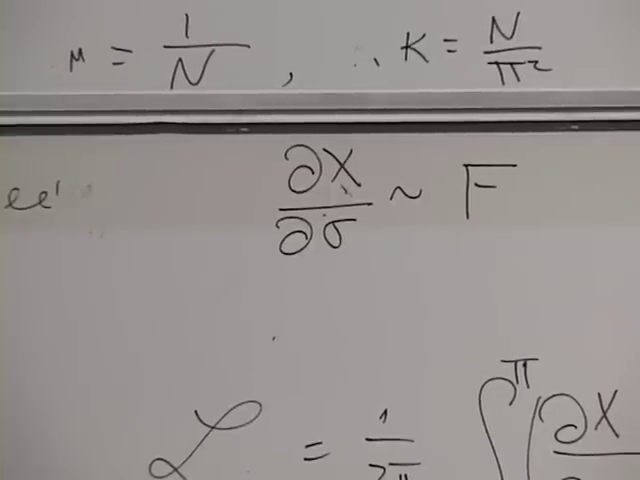
\includegraphics[width=\textwidth]{lecture_02_figure_16.png}
    \par\smallskip\footnotesize (a) 局所的な傾きに比例する端点の力。
  \end{minipage}\hfill
  \begin{minipage}[t]{0.48\textwidth}
    \centering
    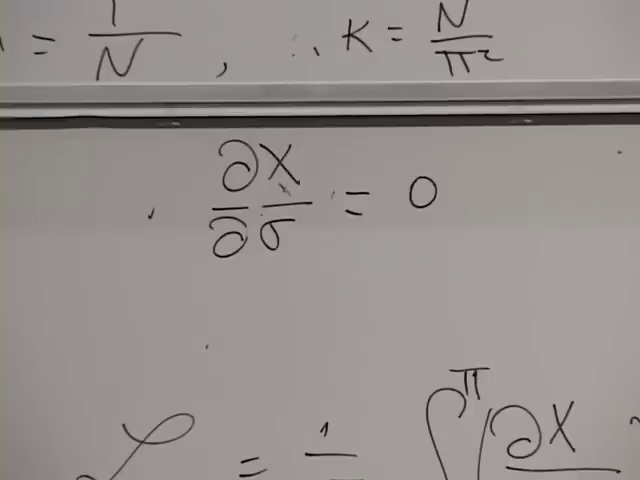
\includegraphics[width=\textwidth]{lecture_02_figure_17.png}
    \par\smallskip\footnotesize (b) 有限加速度の条件。
  \end{minipage}
  \caption{自由端境界条件のニュートン法則による導出。}
  \lectureframe{01:18:20 and 01:20:10}
  \label{fig:l02-neumann-board}
\end{figure}

最後の点に対するニュートンの方程式は

\begin{equation}
  \mu\,\partial_\tau^2X=F_{\mathrm{end}},
  \qquad
  \mu=\frac1N=\frac{\Delta\sigma}{\pi}.
  \label{eq:l02-endpoint-newton}
\end{equation}

\eqref{eq:l02-endpoint-force}と\eqref{eq:l02-endpoint-newton}を組み合わせると、

\begin{equation}
  \partial_\sigma X
  =
  -\Delta\sigma\,\partial_\tau^2X
  \quad\text{at the right endpoint},
  \label{eq:l02-endpoint-scaling}
\end{equation}

左端点では力の符号が逆になる。もし\(\Delta\sigma\to0\)のとき\(\partial_\sigma X\)が非零の定数に近づくなら、端点の加速度は\(N\)のように発散する。したがって、有限の加速度を持つ妥当な連続極限には次が必要である。

\begin{equation}
  \left.\partial_\sigma X\right|_{0,\pi}=0,
  \qquad
  \left.\partial_\sigma Y\right|_{0,\pi}=0.
  \label{eq:l02-open-neumann}
\end{equation}

\begin{figure}[H]
  \centering
  \begin{adjustbox}{max width=\linewidth}
  \begin{tikzpicture}[>=Latex,thick,scale=1.0]
    \coordinate (a) at (0,0);
    \coordinate (b) at (4.5,0.75);
    \filldraw[white] (a) circle (0.12);
    \draw (a) circle (0.12);
    \filldraw[white] (b) circle (0.12);
    \draw (b) circle (0.12);
    \draw[decorate,decoration={zigzag,segment length=6pt,amplitude=3pt}]
      (a) -- (b);
    \draw[dashed] (a) -- (0,-1.2);
    \draw[dashed] (b) -- (4.5,-1.2);
    \draw[<->] (4.85,0) -- (4.85,0.75)
      node[midway,right] {\(\Delta X\)};
    \draw[->,red!70!black] (b) -- (5.75,0.95)
      node[right] {\(F_{\rm end}=-k\Delta X\)};
    \node[below] at (0,-1.2) {\(N-1\)};
    \node[below] at (4.5,-1.2) {\(N\)};
    \node at (2.5,-2.0)
      {\(\mu\ddot X=-k\Delta X
      \ \Longrightarrow\
      \partial_\sigma X=-\Delta\sigma\,\ddot X\to0\)};
  \end{tikzpicture}
  \end{adjustbox}
  \caption{最後の点は正則化極限で質量がゼロになる。有限の加速度が可能なのは、端点の傾きがゼロになるときだけである。}
  \label{fig:l02-neumann-redraw}
\end{figure}

両端および両横方向で同じ議論を行うと、自由な開弦に対するノイマン境界条件が得られる。

\section{開いた弦の基準モード}

これで完全な古典系が得られた。すなわちラグランジアンとその境界条件である。フーリエ解析を行えば量子化は簡単になる。端点がノイマン条件であるから、

\begin{align}
  X(\sigma,\tau)
  &=
  \sum_{n=0}^{\infty}X_n(\tau)\cos(n\sigma),
  \label{eq:l02-X-expansion}\\
  Y(\sigma,\tau)
  &=
  \sum_{n=0}^{\infty}Y_n(\tau)\cos(n\sigma).
  \label{eq:l02-Y-expansion}
\end{align}

余弦関数が\(\sigma\)依存性をすべて含んでいる。係数が時間依存性をすべて含んでおり、弦は\(X_n(\tau)\)と\(Y_n(\tau)\)が変化するために揺れる。

\begin{figure}[H]
  \centering
  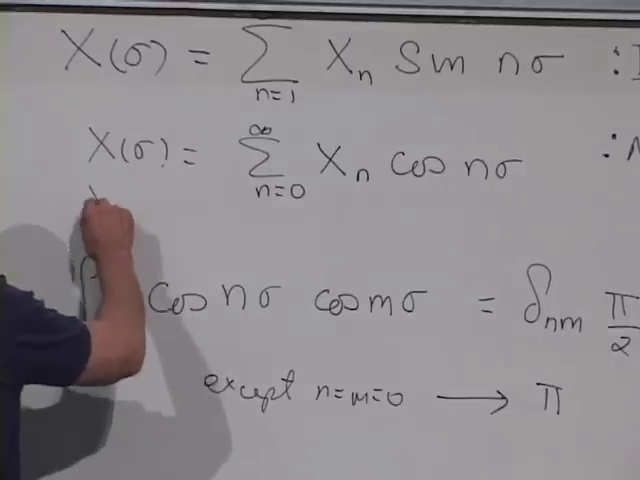
\includegraphics[width=0.78\textwidth]{lecture_02_figure_18.png}
  \caption{ノイマン条件によるモード展開を、二重和を潰す直交性の規則の隣に置いたもの。}
  \lectureframe{01:21:45}
  \label{fig:l02-mode-expansion-board}
\end{figure}

\subsection{運動項とゼロモード}

時間微分を行うと

\begin{equation}
  \partial_\tau X
  =
  \sum_{n=0}^{\infty}\dot X_n(\tau)\cos(n\sigma).
  \label{eq:l02-time-mode}
\end{equation}

二乗すると\(n\)と\(m\)に関する二重和が生じるが、\eqref{eq:l02-cos-orthogonality}が\(n\neq m\)であるすべての項を消す。定数モードを別に扱うと、

\begin{equation}
  \frac{1}{2\pi}\int_0^\pi
  (\partial_\tau X)^2\,d\sigma
  =
  \frac12\dot X_0^{\,2}
  +
  \frac14\sum_{n=1}^{\infty}\dot X_n^{\,2}.
  \label{eq:l02-mode-kinetic}
\end{equation}

\begin{figure}[H]
  \centering
  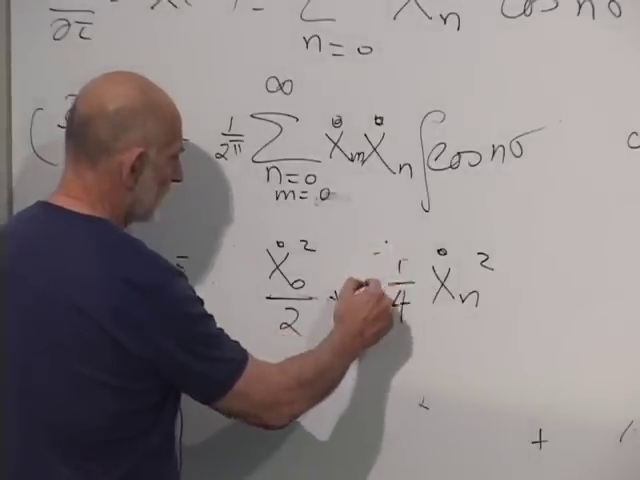
\includegraphics[width=0.76\textwidth]{lecture_02_figure_19.png}
  \caption{直交性の積分により、運動の二重和がゼロモードと対角和に帰着する。}
  \lectureframe{01:29:10}
  \label{fig:l02-mode-kinetic-board}
\end{figure}

定数係数は平均位置であり、

\begin{equation}
  X_0(\tau)=\frac1\pi\int_0^\pi X(\sigma,\tau)\,d\sigma ,
  \label{eq:l02-center-of-mass}
\end{equation}

同様に\(Y_0\)についても成り立つ。一様なアナログ質量密度のもとでは、これらは重心座標である。それらは運動エネルギーをもつが復元力をもたない。弦全体が横平面内を自由に動くことができる。

\subsection{伸長項と振動子の振動数}

空間微分を行うと

\begin{equation}
  \partial_\sigma X
  =
  -\sum_{n=1}^{\infty}nX_n(\tau)\sin(n\sigma).
  \label{eq:l02-spatial-mode}
\end{equation}

一様な並進は弦を伸長させないので、ゼロモードは消える。正弦関数の直交性を用いると、

\begin{equation}
  \frac{1}{2\pi}\int_0^\pi
  (\partial_\sigma X)^2\,d\sigma
  =
  \frac14\sum_{n=1}^{\infty}n^2X_n^{\,2}.
  \label{eq:l02-mode-potential}
\end{equation}

\begin{figure}[H]
  \centering
  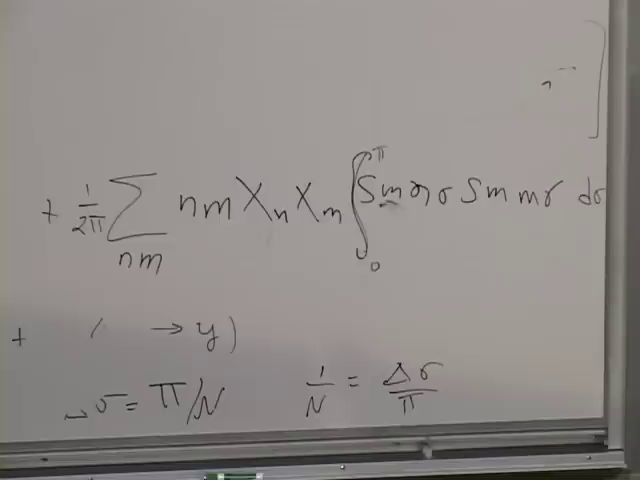
\includegraphics[width=0.76\textwidth]{lecture_02_figure_20.png}
  \caption{余弦級数を微分すると正弦の二重和が生じ、直交性が再び\(n=m\)を強制する。}
  \lectureframe{01:31:40}
  \label{fig:l02-mode-potential-board}
\end{figure}

したがって\(X\)セクターのラグランジアンは

\begin{equation}
  L_X
  =
  \frac12\dot X_0^{\,2}
  +
  \frac14\sum_{n=1}^{\infty}
  \left(
    \dot X_n^{\,2}-n^2X_n^{\,2}
  \right),
  \label{eq:l02-X-lagrangian}
\end{equation}

であり、\(Y\)についても同一の表式が成り立つ。対応するエネルギーでは\(n^2X_n^2\)の前に正符号がつく。すべての非ゼロモードは独立な調和振動子であり、\eqref{eq:l02-oscillator-lagrangian}と比較すると

\begin{equation}
  \omega_n=n,
  \qquad n=1,2,3,\ldots .
  \label{eq:l02-mode-frequency}
\end{equation}

\begin{figure}[H]
  \centering
  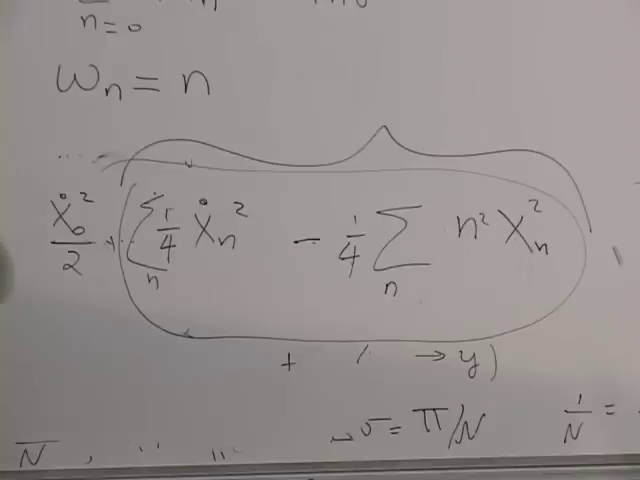
\includegraphics[width=0.80\textwidth]{lecture_02_figure_21.png}
  \caption{分離された振動子のラグランジアンと、結論\(\omega_n=n\)。同一の\(Y\)の塔を以下に示す。}
  \lectureframe{01:35:50}
  \label{fig:l02-oscillator-modes-board}
\end{figure}

基準モードはまさに弦の倍音である。第一のモードはゆっくりと曲がり、第二は二倍の振動数をもち、第三は三倍、以下同様である。自由理論において一つの倍音が別の倍音と結合するのを防ぐのが直交性である。

\begin{classroomqa}
\audiencequestion{\(n=0\)の振動子はどうなったのか。\lecturetimestamp{01:34:49}}
\lecturerresponse{それは内部振動子ではまったくないので振動数がゼロである。それは重心を並進させる。弦全体を特定の横位置に戻すばねは存在しないので、ゼロモードは自由粒子の座標である。}
\end{classroomqa}

重心の運動項を落とすと内部エネルギーが残り、

\begin{equation}
  E_{\mathrm{int}}
  =
  \frac14
  \sum_{n=1}^{\infty}
  \left[
    \dot X_n^{\,2}+n^2X_n^{\,2}
    +\dot Y_n^{\,2}+n^2Y_n^{\,2}
  \right].
  \label{eq:l02-internal-energy}
\end{equation}

光円錐正規化では、これは弦状態の不変質量の二乗に比例する。こうして我々は相対論的な質量の問題を、二つの可算な振動子の塔の量子力学に変換した。

\section{量子化された準位と粒子の振る舞い}

\(a_n^\dagger\)が振動数\(n\)の\(X\)振動子に一つの量子を生成し、\(b_n^\dagger\)が\(Y\)について同じことを行うものとする。講義では系統的な演算子の扱いは後回しにされるが、この記法により準位の数え方が透明になる。基底状態のオフセットを基準にすると、

\begin{equation}
  \begin{aligned}
    \Delta E_{\mathrm{int}}
    &=\sum_{n=1}^{\infty}n\left(Q_n^X+Q_n^Y\right),\\
    Q_n^X,Q_n^Y&\in\{0,1,2,\ldots\}.
  \end{aligned}
  \label{eq:l02-quantized-energy}
\end{equation}

ここで\(\hbar=1\)である。整数\(n\)はどの振動子が励起されているかを示し、\(Q_n\)はそこに何個の量子が入っているかを数える。\editorialnote{各振動子は零点エネルギーにも寄与する。この無限和は正則化を必要とし、弦の質量公式の切片を与える。講義ではここで基底状態のオフセットを意図的に未指定のままにし、励起準位のみを数えている。}

振動子の真空\(\ket{0}\)は空の時空ではない。それは内部振動子が励起されていない一つの開いた弦である。それはエネルギー、運動量、そして弦スペクトルにおける確定した位置をもつ。

第一準位には二つの状態があり、

\begin{equation}
  a_1^\dagger\ket{0},
  \qquad
  b_1^\dagger\ket{0},
  \label{eq:l02-level-one}
\end{equation}

これらは\(X\)または\(Y\)に沿って偏極した最低次の倍音に対応する。線形結合は任意の横偏極を表す。

第二準位には五つの状態がある。

\begin{equation}
  (a_1^\dagger)^2\ket{0},
  \quad
  a_1^\dagger b_1^\dagger\ket{0},
  \quad
  (b_1^\dagger)^2\ket{0},
  \quad
  a_2^\dagger\ket{0},
  \quad
  b_2^\dagger\ket{0}.
  \label{eq:l02-level-two}
\end{equation}

三つは第一倍音の二つの量子を用い、二つは第二倍音の一つの量子を用いる。どちらの構成も二単位のコストがかかる。

\begin{figure}[H]
  \centering
  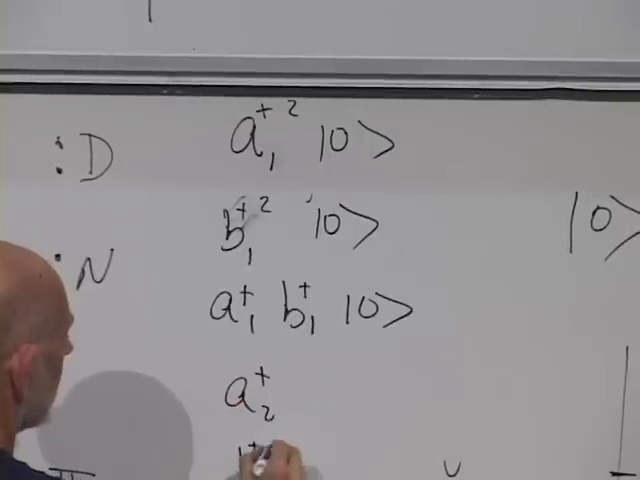
\includegraphics[width=0.76\textwidth]{lecture_02_figure_22.png}
  \caption{聴衆からの異議の後で数え直された第二準位の五つの状態。二つの二重励起、一つの混合励起、そして二つの第二倍音励起である。}
  \lectureframe{01:44:00}
  \label{fig:l02-levels-board}
\end{figure}

\begin{figure}[H]
  \centering
  \begin{adjustbox}{max width=\linewidth}
  \begin{tikzpicture}[>=Latex,thick]
    \draw[->] (0,0) -- (0,5.1) node[above] {\(\Delta E_{\rm int}\)};
    \draw[blue!70!black] (-0.65,0.55) -- (0.65,0.55);
    \node[right] at (0.85,0.55) {\(\ket{0}\) \quad multiplicity \(1\)};
    \draw[blue!70!black] (-0.65,2.15) -- (0.65,2.15);
    \node[right] at (0.85,2.15)
      {\(a_1^\dagger\ket{0},\ b_1^\dagger\ket{0}\)
      \quad multiplicity \(2\)};
    \draw[blue!70!black] (-0.65,3.75) -- (0.65,3.75);
    \node[right,text width=8.6cm] at (0.85,3.75)
      {\((a_1^\dagger)^2\ket{0},
      a_1^\dagger b_1^\dagger\ket{0},
      (b_1^\dagger)^2\ket{0},
      a_2^\dagger\ket{0},\ b_2^\dagger\ket{0}\)
      \quad multiplicity \(5\)};
    \node[left] at (-0.75,0.55) {\(0\)};
    \node[left] at (-0.75,2.15) {\(1\)};
    \node[left] at (-0.75,3.75) {\(2\)};
  \end{tikzpicture}
  \end{adjustbox}
  \caption{二つの横方向をもつ開いた弦の最初の三つの励起準位。}
  \label{fig:l02-levels-redraw}
\end{figure}

\begin{classroomqa}
\audiencequestion{第2励起準位には4つの状態があるのか、それとも5つか。\lecturetimestamp{01:43:04}}
\lecturerresponse{5つである。\(X_1\)を2回励起し、\(Y_1\)を2回励起し、それぞれを1回ずつ励起すると3つの状態が得られる。\(X_2\)を1回、または\(Y_2\)を1回励起するとさらに2つが得られる。提案された演習は、次の2つの準位を数え上げることである。}
\end{classroomqa}

本質的な結論はすでに見えている。連続する準位は有限の間隔で隔てられており、それぞれが有限の多重度をもつ。したがって、量子化された弦は、コーヒーや気体、あるいは普通のヴァイオリン弦と区別するスペクトルの判定基準によって、粒子様である。後に、どの状態が物理的に許容され、どの病的な状態を除去しなければならないかを決定する。

\section{なぜ開弦の相互作用は閉弦を生じるのか}

開弦には2つの端点がある。その基本的な相互作用は弦を結合させたり分裂させたりする。ハドロン的描像では、一方の端にクォーク、他方の端に反クォークを想像してよい。それらの対消滅が2つの弦の断片を結合させる。後に興味の対象となる基本弦は、そのような文字通りのハドロン的端点解釈を担う必要はないが、局所的な結合規則はそのまま残る。

ここで、1本の開弦が揺らぎ、その自身の端点同士が近づくまでを考えよう。局所的には、一方の端点は、他方の端点が別の弦ではなく同じ弦に属していることを知り得ない。端点がそもそも結合してよいのであれば、ここでも結合してよく、閉じたループを生じる。

\begin{figure}[H]
  \centering
  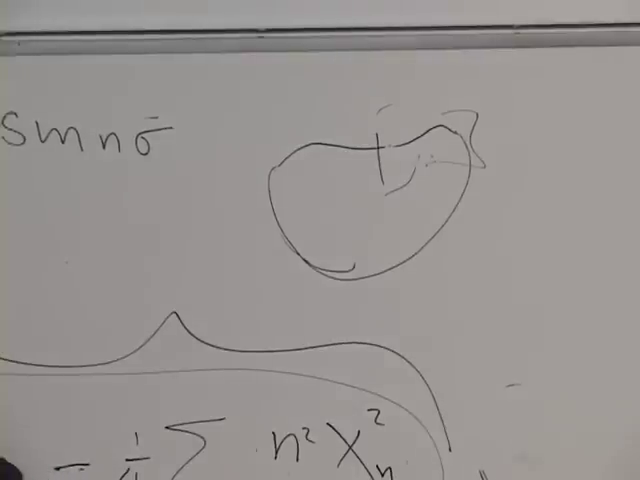
\includegraphics[width=0.70\textwidth]{lecture_02_figure_23.png}
  \caption{開弦が揺らぎ、その2つの端点が出会って閉じたループを形成するまでの黒板スケッチ。}
  \lectureframe{01:47:00}
  \label{fig:l02-closed-board}
\end{figure}

\begin{figure}[H]
  \centering
  \begin{adjustbox}{max width=\linewidth}
  \begin{tikzpicture}[>=Latex,thick]
    \begin{scope}
      \draw[blue!70!black]
        (0,0) .. controls (0.8,1.2) and (1.7,-1.0) .. (2.6,0.45)
        .. controls (3.4,1.55) and (4.0,0.3) .. (4.7,0.85);
      \fill (0,0) circle (0.09);
      \fill (4.7,0.85) circle (0.09);
      \node at (2.35,-1.25) {open string fluctuation};
    \end{scope}
    \draw[->,line width=1pt] (5.25,0.3) -- (6.65,0.3)
      node[midway,above] {join};
    \begin{scope}[xshift=8.1cm]
      \draw[orange!85!black]
        (0,0) .. controls (0.3,1.5) and (2.5,1.8) .. (3.1,0.3)
        .. controls (3.5,-1.1) and (0.7,-1.5) .. (0,0);
      \node at (1.55,-1.85) {closed string};
    \end{scope}
  \end{tikzpicture}
  \end{adjustbox}
  \caption{端点の結合が許されれば、開弦はそれ自身で閉じることができる。}
  \label{fig:l02-closed-redraw}
\end{figure}

したがって、理論は開弦をもたずに閉弦を含むことはあり得るが、開弦をもつ相互作用する理論は閉弦を一貫して避けることはできない。この非対称性が重要な予言である。スペクトルの同定は後に展開されるが、行き先はすでに見えている。質量ゼロの開弦状態はしばしば光子のようなゲージ粒子を与え、一方、閉弦のスペクトルは質量ゼロのスピン2の状態、すなわちグラビトンを含む。弦理論が相互作用するものである以上、閉弦、したがって重力は、任意の装飾ではない。
